\batchmode


\documentclass{book}
\RequirePackage{ifthen}




\usepackage[dvips]{graphicx}
\usepackage{amsmath}
\usepackage{bm}
\usepackage{times}
\usepackage{txfonts}
\usepackage{mathrsfs}




\usepackage[dvips]{color}


\pagecolor[gray]{.7}

\usepackage[latin1]{inputenc}



\makeatletter

\makeatletter
\count@=\the\catcode`\_ \catcode`\_=8 
\newenvironment{tex2html_wrap}{}{}%
\catcode`\<=12\catcode`\_=\count@
\newcommand{\providedcommand}[1]{\expandafter\providecommand\csname #1\endcsname}%
\newcommand{\renewedcommand}[1]{\expandafter\providecommand\csname #1\endcsname{}%
  \expandafter\renewcommand\csname #1\endcsname}%
\newcommand{\newedenvironment}[1]{\newenvironment{#1}{}{}\renewenvironment{#1}}%
\let\newedcommand\renewedcommand
\let\renewedenvironment\newedenvironment
\makeatother
\let\mathon=$
\let\mathoff=$
\ifx\AtBeginDocument\undefined \newcommand{\AtBeginDocument}[1]{}\fi
\newbox\sizebox
\setlength{\hoffset}{0pt}\setlength{\voffset}{0pt}
\addtolength{\textheight}{\footskip}\setlength{\footskip}{0pt}
\addtolength{\textheight}{\topmargin}\setlength{\topmargin}{0pt}
\addtolength{\textheight}{\headheight}\setlength{\headheight}{0pt}
\addtolength{\textheight}{\headsep}\setlength{\headsep}{0pt}
\setlength{\textwidth}{451pt}
\setlength{\textheight}{554pt}
\newwrite\lthtmlwrite
\makeatletter
\let\realnormalsize=\normalsize
\global\topskip=2sp
\def\preveqno{}\let\real@float=\@float \let\realend@float=\end@float
\def\@float{\let\@savefreelist\@freelist\real@float}
\def\liih@math{\ifmmode$\else\bad@math\fi}
\def\end@float{\realend@float\global\let\@freelist\@savefreelist}
\let\real@dbflt=\@dbflt \let\end@dblfloat=\end@float
\let\@largefloatcheck=\relax
\let\if@boxedmulticols=\iftrue
\def\@dbflt{\let\@savefreelist\@freelist\real@dbflt}
\def\adjustnormalsize{\def\normalsize{\mathsurround=0pt \realnormalsize
 \parindent=0pt\abovedisplayskip=0pt\belowdisplayskip=0pt}%
 \def\phantompar{\csname par\endcsname}\normalsize}%
\def\lthtmltypeout#1{{\let\protect\string \immediate\write\lthtmlwrite{#1}}}%
\newcommand\lthtmlhboxmathA{\adjustnormalsize\setbox\sizebox=\hbox\bgroup\kern.05em }%
\newcommand\lthtmlhboxmathB{\adjustnormalsize\setbox\sizebox=\hbox to\hsize\bgroup\hfill }%
\newcommand\lthtmlvboxmathA{\adjustnormalsize\setbox\sizebox=\vbox\bgroup %
 \let\ifinner=\iffalse \let\)\liih@math }%
\newcommand\lthtmlboxmathZ{\@next\next\@currlist{}{\def\next{\voidb@x}}%
 \expandafter\box\next\egroup}%
\newcommand\lthtmlmathtype[1]{\gdef\lthtmlmathenv{#1}}%
\newcommand\lthtmllogmath{\lthtmltypeout{l2hSize %
:\lthtmlmathenv:\the\ht\sizebox::\the\dp\sizebox::\the\wd\sizebox.\preveqno}}%
\newcommand\lthtmlfigureA[1]{\let\@savefreelist\@freelist
       \lthtmlmathtype{#1}\lthtmlvboxmathA}%
\newcommand\lthtmlpictureA{\bgroup\catcode`\_=8 \lthtmlpictureB}%
\newcommand\lthtmlpictureB[1]{\lthtmlmathtype{#1}\egroup
       \let\@savefreelist\@freelist \lthtmlhboxmathB}%
\newcommand\lthtmlpictureZ[1]{\hfill\lthtmlfigureZ}%
\newcommand\lthtmlfigureZ{\lthtmlboxmathZ\lthtmllogmath\copy\sizebox
       \global\let\@freelist\@savefreelist}%
\newcommand\lthtmldisplayA{\bgroup\catcode`\_=8 \lthtmldisplayAi}%
\newcommand\lthtmldisplayAi[1]{\lthtmlmathtype{#1}\egroup\lthtmlvboxmathA}%
\newcommand\lthtmldisplayB[1]{\edef\preveqno{(\theequation)}%
  \lthtmldisplayA{#1}\let\@eqnnum\relax}%
\newcommand\lthtmldisplayZ{\lthtmlboxmathZ\lthtmllogmath\lthtmlsetmath}%
\newcommand\lthtmlinlinemathA{\bgroup\catcode`\_=8 \lthtmlinlinemathB}
\newcommand\lthtmlinlinemathB[1]{\lthtmlmathtype{#1}\egroup\lthtmlhboxmathA
  \vrule height1.5ex width0pt }%
\newcommand\lthtmlinlineA{\bgroup\catcode`\_=8 \lthtmlinlineB}%
\newcommand\lthtmlinlineB[1]{\lthtmlmathtype{#1}\egroup\lthtmlhboxmathA}%
\newcommand\lthtmlinlineZ{\egroup\expandafter\ifdim\dp\sizebox>0pt %
  \expandafter\centerinlinemath\fi\lthtmllogmath\lthtmlsetinline}
\newcommand\lthtmlinlinemathZ{\egroup\expandafter\ifdim\dp\sizebox>0pt %
  \expandafter\centerinlinemath\fi\lthtmllogmath\lthtmlsetmath}
\newcommand\lthtmlindisplaymathZ{\egroup %
  \centerinlinemath\lthtmllogmath\lthtmlsetmath}
\def\lthtmlsetinline{\hbox{\vrule width.1em \vtop{\vbox{%
  \kern.1em\copy\sizebox}\ifdim\dp\sizebox>0pt\kern.1em\else\kern.3pt\fi
  \ifdim\hsize>\wd\sizebox \hrule depth1pt\fi}}}
\def\lthtmlsetmath{\hbox{\vrule width.1em\kern-.05em\vtop{\vbox{%
  \kern.1em\kern0.8 pt\hbox{\hglue.17em\copy\sizebox\hglue0.8 pt}}\kern.3pt%
  \ifdim\dp\sizebox>0pt\kern.1em\fi \kern0.8 pt%
  \ifdim\hsize>\wd\sizebox \hrule depth1pt\fi}}}
\def\centerinlinemath{%
  \dimen1=\ifdim\ht\sizebox<\dp\sizebox \dp\sizebox\else\ht\sizebox\fi
  \advance\dimen1by.5pt \vrule width0pt height\dimen1 depth\dimen1 
 \dp\sizebox=\dimen1\ht\sizebox=\dimen1\relax}

\def\lthtmlcheckvsize{\ifdim\ht\sizebox<\vsize 
  \ifdim\wd\sizebox<\hsize\expandafter\hfill\fi \expandafter\vfill
  \else\expandafter\vss\fi}%
\providecommand{\selectlanguage}[1]{}%
\makeatletter \tracingstats = 1 
\providecommand{\Beta}{\textrm{B}}
\providecommand{\Mu}{\textrm{M}}
\providecommand{\Kappa}{\textrm{K}}
\providecommand{\Rho}{\textrm{R}}
\providecommand{\Epsilon}{\textrm{E}}
\providecommand{\Chi}{\textrm{X}}
\providecommand{\Iota}{\textrm{J}}
\providecommand{\omicron}{\textrm{o}}
\providecommand{\Zeta}{\textrm{Z}}
\providecommand{\Eta}{\textrm{H}}
\providecommand{\Nu}{\textrm{N}}
\providecommand{\Omicron}{\textrm{O}}
\providecommand{\Tau}{\textrm{T}}
\providecommand{\Alpha}{\textrm{A}}


\begin{document}
\pagestyle{empty}\thispagestyle{empty}\lthtmltypeout{}%
\lthtmltypeout{latex2htmlLength hsize=\the\hsize}\lthtmltypeout{}%
\lthtmltypeout{latex2htmlLength vsize=\the\vsize}\lthtmltypeout{}%
\lthtmltypeout{latex2htmlLength hoffset=\the\hoffset}\lthtmltypeout{}%
\lthtmltypeout{latex2htmlLength voffset=\the\voffset}\lthtmltypeout{}%
\lthtmltypeout{latex2htmlLength topmargin=\the\topmargin}\lthtmltypeout{}%
\lthtmltypeout{latex2htmlLength topskip=\the\topskip}\lthtmltypeout{}%
\lthtmltypeout{latex2htmlLength headheight=\the\headheight}\lthtmltypeout{}%
\lthtmltypeout{latex2htmlLength headsep=\the\headsep}\lthtmltypeout{}%
\lthtmltypeout{latex2htmlLength parskip=\the\parskip}\lthtmltypeout{}%
\lthtmltypeout{latex2htmlLength oddsidemargin=\the\oddsidemargin}\lthtmltypeout{}%
\makeatletter
\if@twoside\lthtmltypeout{latex2htmlLength evensidemargin=\the\evensidemargin}%
\else\lthtmltypeout{latex2htmlLength evensidemargin=\the\oddsidemargin}\fi%
\lthtmltypeout{}%
\makeatother
\setcounter{page}{1}
\onecolumn

% !!! IMAGES START HERE !!!

{\newpage\clearpage
\lthtmlinlinemathA{tex2html_wrap_inline3422}%
$ \xi $%
\lthtmlinlinemathZ
\lthtmlcheckvsize\clearpage}

{\newpage\clearpage
\lthtmlinlinemathA{tex2html_wrap_inline3424}%
$ R_T$%
\lthtmlinlinemathZ
\lthtmlcheckvsize\clearpage}

{\newpage\clearpage
\lthtmlinlinemathA{tex2html_wrap_inline3434}%
$ \delimiter "426830A $%
\lthtmlinlinemathZ
\lthtmlcheckvsize\clearpage}

{\newpage\clearpage
\lthtmlinlinemathA{tex2html_wrap_inline3436}%
$ \delimiter "526930B $%
\lthtmlinlinemathZ
\lthtmlcheckvsize\clearpage}

{\newpage\clearpage
\lthtmlinlinemathA{tex2html_wrap_inline3466}%
$ \bm  {A}\cdot \bm  {x}$%
\lthtmlinlinemathZ
\lthtmlcheckvsize\clearpage}

\stepcounter{chapter}
\stepcounter{chapter}
\stepcounter{section}
{\newpage\clearpage
\lthtmlinlinemathA{tex2html_wrap_inline3494}%
$ \mu$%
\lthtmlinlinemathZ
\lthtmlcheckvsize\clearpage}

\stepcounter{subsection}
\stepcounter{subsection}
{\newpage\clearpage
\lthtmlinlinemathA{tex2html_wrap_inline3498}%
$ \bm{u}^\infty$%
\lthtmlinlinemathZ
\lthtmlcheckvsize\clearpage}

{\newpage\clearpage
\lthtmlinlinemathA{tex2html_wrap_inline3500}%
$ \bm{\Omega}^\infty$%
\lthtmlinlinemathZ
\lthtmlcheckvsize\clearpage}

{\newpage\clearpage
\lthtmlinlinemathA{tex2html_wrap_inline3502}%
$ \bm{E}^\infty$%
\lthtmlinlinemathZ
\lthtmlcheckvsize\clearpage}

{\newpage\clearpage
\lthtmlinlinemathA{tex2html_wrap_inline3504}%
$ {\tt shear-mode} \ne 0$%
\lthtmlinlinemathZ
\lthtmlcheckvsize\clearpage}

{\newpage\clearpage
\lthtmlinlinemathA{tex2html_wrap_inline3510}%
$ \bm{F}_{\text{ext}}$%
\lthtmlinlinemathZ
\lthtmlcheckvsize\clearpage}

{\newpage\clearpage
\lthtmlinlinemathA{tex2html_wrap_inline3512}%
$ \bm{T}_{\text{ext}}$%
\lthtmlinlinemathZ
\lthtmlcheckvsize\clearpage}

{\newpage\clearpage
\lthtmlinlinemathA{tex2html_wrap_inline3514}%
$ \widetilde{\text{St}}$%
\lthtmlinlinemathZ
\lthtmlcheckvsize\clearpage}

{\newpage\clearpage
\lthtmlinlinemathA{tex2html_wrap_inline3520}%
$ \bm{u}^{\infty}$%
\lthtmlinlinemathZ
\lthtmlcheckvsize\clearpage}

{\newpage\clearpage
\lthtmlinlinemathA{tex2html_wrap_inline3522}%
$ \bm{U}^{\infty}$%
\lthtmlinlinemathZ
\lthtmlcheckvsize\clearpage}

{\newpage\clearpage
\lthtmlinlinemathA{tex2html_wrap_inline3524}%
$ \bm{\Omega}^{\infty}$%
\lthtmlinlinemathZ
\lthtmlcheckvsize\clearpage}

{\newpage\clearpage
\lthtmlinlinemathA{tex2html_wrap_inline3526}%
$ \bm{E}^{\infty}$%
\lthtmlinlinemathZ
\lthtmlcheckvsize\clearpage}

{\newpage\clearpage
\lthtmlinlinemathA{tex2html_wrap_indisplay3528}%
$\displaystyle \bm{u}^{\infty}(\bm{x})   =   \bm{U}^{\infty}   +   \bm{\Omega}^{\infty}\times\bm{x}   +   \bm{E}\cdot\bm{x}   .$%
\lthtmlindisplaymathZ
\lthtmlcheckvsize\clearpage}

{\newpage\clearpage
\lthtmlinlinemathA{tex2html_wrap_inline3530}%
$ \bm{\nabla}\bm{u}^{\infty}$%
\lthtmlinlinemathZ
\lthtmlcheckvsize\clearpage}

{\newpage\clearpage
\lthtmlinlinemathA{tex2html_wrap_indisplay3532}%
$\displaystyle \bm{\nabla}\bm{u}^{\infty}   =   \left[     \begin{array}{ccc}       E^{\infty}_{xx} & E^{\infty}_{xy}+\Omega^{\infty}_{z} & E^{\infty}_{xz}-\Omega^{\infty}_{y} \\E^{\infty}_{xy}-\Omega^{\infty}_{z} & E^{\infty}_{yy} & E^{\infty}_{yz}+\Omega^{\infty}_{x} \\E^{\infty}_{xz}+\Omega^{\infty}_{y} & E^{\infty}_{yz}-\Omega^{\infty}_{x} & 1-E^{\infty}_{xx}-E^{\infty}_{yy}     \end{array}   \right]   .$%
\lthtmlindisplaymathZ
\lthtmlcheckvsize\clearpage}

{\newpage\clearpage
\lthtmlinlinemathA{tex2html_wrap_indisplay3534}%
$\displaystyle {\tt Oi}   =   \left(\Omega^{\infty}_{x}, \Omega^{\infty}_{y}, \Omega^{\infty}_{z}\right)   ,$%
\lthtmlindisplaymathZ
\lthtmlcheckvsize\clearpage}

{\newpage\clearpage
\lthtmlinlinemathA{tex2html_wrap_indisplay3536}%
$\displaystyle {\tt Ei}   =   \left(     E^{\infty}_{xx},     E^{\infty}_{xy},     E^{\infty}_{xz},     E^{\infty}_{yz},     E^{\infty}_{yy}   \right)   .$%
\lthtmlindisplaymathZ
\lthtmlcheckvsize\clearpage}

{\newpage\clearpage
\lthtmlinlinemathA{tex2html_wrap_indisplay3540}%
$\displaystyle E^{\infty}_{ij} = E^{\infty}_{ji},\quad   E^{\infty}_{ii} = 0.$%
\lthtmlindisplaymathZ
\lthtmlcheckvsize\clearpage}

{\newpage\clearpage
\lthtmlinlinemathA{tex2html_wrap_inline3542}%
$ xz$%
\lthtmlinlinemathZ
\lthtmlcheckvsize\clearpage}

{\newpage\clearpage
\lthtmlinlinemathA{tex2html_wrap_inline3544}%
$ x$%
\lthtmlinlinemathZ
\lthtmlcheckvsize\clearpage}

{\newpage\clearpage
\lthtmlinlinemathA{tex2html_wrap_inline3546}%
$ y$%
\lthtmlinlinemathZ
\lthtmlcheckvsize\clearpage}

{\newpage\clearpage
\lthtmlinlinemathA{tex2html_wrap_indisplay3548}%
$\displaystyle \Omega^{\infty}_{y} = \frac{1}{2}\dot{\gamma},\quad   E^{\infty}_{xz} = \frac{1}{2}\dot{\gamma},$%
\lthtmlindisplaymathZ
\lthtmlcheckvsize\clearpage}

{\newpage\clearpage
\lthtmlinlinemathA{tex2html_wrap_indisplay3550}%
$\displaystyle \bm{\nabla}\bm{u}^{\infty}   =   \left[     \begin{array}{ccc}       0 & 0 & 0 \\0 & 0 & 0 \\\dot{\gamma} & 0 & 0     \end{array}   \right]   .$%
\lthtmlindisplaymathZ
\lthtmlcheckvsize\clearpage}

{\newpage\clearpage
\lthtmlinlinemathA{tex2html_wrap_indisplay3553}%
$\displaystyle {\tt Oi}$%
\lthtmlindisplaymathZ
\lthtmlcheckvsize\clearpage}

{\newpage\clearpage
\lthtmlinlinemathA{tex2html_wrap_indisplay3555}%
$\displaystyle =$%
\lthtmlindisplaymathZ
\lthtmlcheckvsize\clearpage}

{\newpage\clearpage
\lthtmlinlinemathA{tex2html_wrap_indisplay3557}%
$\displaystyle \left(0, \dot{\gamma}/2, 0\right),$%
\lthtmlindisplaymathZ
\lthtmlcheckvsize\clearpage}

{\newpage\clearpage
\lthtmlinlinemathA{tex2html_wrap_indisplay3559}%
$\displaystyle {\tt Ei}$%
\lthtmlindisplaymathZ
\lthtmlcheckvsize\clearpage}

{\newpage\clearpage
\lthtmlinlinemathA{tex2html_wrap_indisplay3563}%
$\displaystyle \left(
0,
0,
\dot{\gamma}/2,
0,
0
\right)
.$%
\lthtmlindisplaymathZ
\lthtmlcheckvsize\clearpage}

{\newpage\clearpage
\lthtmlinlinemathA{tex2html_wrap_indisplay3567}%
$\displaystyle \bm{\nabla}\bm{u}^{\infty}   =   \left[     \begin{array}{ccc}       \dot{\epsilon} & 0 & 0 \\0 & 0 & 0 \\0 & 0 & -\dot{\epsilon}     \end{array}   \right]   ,$%
\lthtmlindisplaymathZ
\lthtmlcheckvsize\clearpage}

{\newpage\clearpage
\lthtmlinlinemathA{tex2html_wrap_indisplay3569}%
$\displaystyle E^{\infty}_{xx} = -E^{\infty}_{zz} = \dot{\epsilon},$%
\lthtmlindisplaymathZ
\lthtmlcheckvsize\clearpage}

{\newpage\clearpage
\lthtmlinlinemathA{tex2html_wrap_inline3571}%
$ E^{\infty}_{yy} = 1-E^{\infty}_{xx}-E^{\infty}_{zz} = 0$%
\lthtmlinlinemathZ
\lthtmlcheckvsize\clearpage}

{\newpage\clearpage
\lthtmlinlinemathA{tex2html_wrap_indisplay3578}%
$\displaystyle \left(0, 0, 0\right),$%
\lthtmlindisplaymathZ
\lthtmlcheckvsize\clearpage}

{\newpage\clearpage
\lthtmlinlinemathA{tex2html_wrap_indisplay3584}%
$\displaystyle \left(
\dot{\epsilon},
0,
0,
0,
0
\right)
.$%
\lthtmlindisplaymathZ
\lthtmlcheckvsize\clearpage}

\stepcounter{subsection}
\stepcounter{subsubsection}
{\newpage\clearpage
\lthtmlinlinemathA{tex2html_wrap_inline3588}%
$ (a_{i}+a_{j})\  {\tt *\  rmin}$%
\lthtmlinlinemathZ
\lthtmlcheckvsize\clearpage}

{\newpage\clearpage
\lthtmlinlinemathA{tex2html_wrap_inline3590}%
$ T_r/T_k$%
\lthtmlinlinemathZ
\lthtmlcheckvsize\clearpage}

\stepcounter{subsubsection}
\stepcounter{subsection}
\stepcounter{subsubsection}
{\newpage\clearpage
\lthtmlinlinemathA{tex2html_wrap_indisplay3595}%
$\displaystyle \frac{{\rm d}\bm{x}}{{\rm d}t}   =   \bm{U}   ,$%
\lthtmlindisplaymathZ
\lthtmlcheckvsize\clearpage}

{\newpage\clearpage
\lthtmlinlinemathA{tex2html_wrap_inline3597}%
$ \bm{U}$%
\lthtmlinlinemathZ
\lthtmlcheckvsize\clearpage}

{\newpage\clearpage
\lthtmlinlinemathA{tex2html_wrap_indisplay3601}%
$\displaystyle \bm{U}   =   \bm{M}\cdot\bm{F}_{\text{ext}}   ,$%
\lthtmlindisplaymathZ
\lthtmlcheckvsize\clearpage}

\stepcounter{subsubsection}
{\newpage\clearpage
\lthtmlinlinemathA{tex2html_wrap_indisplay3607}%
$\displaystyle \widetilde{\text{St}}\ 
\frac{{\rm d}\bm{U}}{{\rm d}t}$%
\lthtmlindisplaymathZ
\lthtmlcheckvsize\clearpage}

{\newpage\clearpage
\lthtmlinlinemathA{tex2html_wrap_indisplay3611}%
$\displaystyle -\bm{U}+\bm{V}
,$%
\lthtmlindisplaymathZ
\lthtmlcheckvsize\clearpage}

{\newpage\clearpage
\lthtmlinlinemathA{tex2html_wrap_indisplay3613}%
$\displaystyle \frac{{\rm d}\bm{x}}{{\rm d}t}$%
\lthtmlindisplaymathZ
\lthtmlcheckvsize\clearpage}

{\newpage\clearpage
\lthtmlinlinemathA{tex2html_wrap_indisplay3617}%
$\displaystyle \bm{U}
,$%
\lthtmlindisplaymathZ
\lthtmlcheckvsize\clearpage}

{\newpage\clearpage
\lthtmlinlinemathA{tex2html_wrap_inline3623}%
$ \bm{V}$%
\lthtmlinlinemathZ
\lthtmlcheckvsize\clearpage}

{\newpage\clearpage
\lthtmlinlinemathA{tex2html_wrap_indisplay3625}%
$\displaystyle \bm{V}   =   \bm{M}\cdot\bm{F}_{\text{ext}}   .$%
\lthtmlindisplaymathZ
\lthtmlcheckvsize\clearpage}

\stepcounter{paragraph}
{\newpage\clearpage
\lthtmlinlinemathA{tex2html_wrap_indisplay3630}%
$\displaystyle \frac{{\rm d}\bm{U}}{{\rm d}t}   =   -\bm{F}_{\text{stokes}}   +\bm{F}_{\text{ext}}   ,$%
\lthtmlindisplaymathZ
\lthtmlcheckvsize\clearpage}

{\newpage\clearpage
\lthtmlinlinemathA{tex2html_wrap_inline3633}%
$ \bm{F}_{\text{stokes}} = \bm{R}\cdot\bm{U}$%
\lthtmlinlinemathZ
\lthtmlcheckvsize\clearpage}

\stepcounter{subsubsection}
{\newpage\clearpage
\lthtmlinlinemathA{tex2html_wrap_inline3636}%
$ \epsilon$%
\lthtmlinlinemathZ
\lthtmlcheckvsize\clearpage}

\stepcounter{subsection}
\stepcounter{subsection}
\stepcounter{subsubsection}
\stepcounter{subsubsection}
\stepcounter{subsubsection}
\stepcounter{subsection}
\stepcounter{subsubsection}
\stepcounter{subsubsection}
\stepcounter{subsubsection}
\stepcounter{subsection}
\stepcounter{subsection}
\stepcounter{section}
{\newpage\clearpage
\lthtmlinlinemathA{tex2html_wrap_indisplay3653}%
$\displaystyle 6\pi\mu a
\bm{U}^\alpha$%
\lthtmlindisplaymathZ
\lthtmlcheckvsize\clearpage}

{\newpage\clearpage
\lthtmlinlinemathA{tex2html_wrap_indisplay3657}%
$\displaystyle \bm{F}^\alpha
+
\sum_{\gamma}
{\sum_{\beta}}'
\bm{M}(\bm{r}_{\beta\alpha} + \bm{r}_\gamma)
\cdot\bm{F}^\beta$%
\lthtmlindisplaymathZ
\lthtmlcheckvsize\clearpage}

{\newpage\clearpage
\lthtmlinlinemathA{tex2html_wrap_indisplay3661}%
$\displaystyle \bm{F}^\alpha$%
\lthtmlindisplaymathZ
\lthtmlcheckvsize\clearpage}

{\newpage\clearpage
\lthtmlinlinemathA{tex2html_wrap_indisplay3663}%
$\displaystyle +
\sum_{\gamma}
{\sum_{\beta\neq\alpha}}'
\bm{M}^{\rm real}(\bm{r}_{\beta\alpha} + \bm{r}_\gamma)
\cdot\bm{F}^\beta$%
\lthtmlindisplaymathZ
\lthtmlcheckvsize\clearpage}

{\newpage\clearpage
\lthtmlinlinemathA{tex2html_wrap_indisplay3665}%
$\displaystyle +
\frac{1}{V}
\sum_{\lambda}
\sum_{\beta = 1}^{N}
\cos(\bm{k}_\lambda\cdot\bm{r}_{\beta\alpha})\ 
\tilde{\bm{M}}^{\rm recip}(\bm{k}_\lambda)
\cdot\bm{F}^\beta$%
\lthtmlindisplaymathZ
\lthtmlcheckvsize\clearpage}

{\newpage\clearpage
\lthtmlinlinemathA{tex2html_wrap_indisplay3667}%
$\displaystyle -
\bm{M}^{\rm recip}(\bm{r} = \bm{0})
\cdot\bm{F}^\alpha
,$%
\lthtmlindisplaymathZ
\lthtmlcheckvsize\clearpage}

{\newpage\clearpage
\lthtmlinlinemathA{tex2html_wrap_inline3669}%
$ \gamma$%
\lthtmlinlinemathZ
\lthtmlcheckvsize\clearpage}

{\newpage\clearpage
\lthtmlinlinemathA{tex2html_wrap_inline3671}%
$ \bm{r}_\gamma = (n_x l_x, n_y l_y, n_z l_z)^\dagger$%
\lthtmlinlinemathZ
\lthtmlcheckvsize\clearpage}

{\newpage\clearpage
\lthtmlinlinemathA{tex2html_wrap_inline3673}%
$ (n_x, n_y, n_z)$%
\lthtmlinlinemathZ
\lthtmlcheckvsize\clearpage}

{\newpage\clearpage
\lthtmlinlinemathA{tex2html_wrap_inline3675}%
$ \bm{r}_{\beta\alpha} = \bm{x}^\alpha - \bm{x}^\beta$%
\lthtmlinlinemathZ
\lthtmlcheckvsize\clearpage}

{\newpage\clearpage
\lthtmlinlinemathA{tex2html_wrap_inline3677}%
$ \beta$%
\lthtmlinlinemathZ
\lthtmlcheckvsize\clearpage}

{\newpage\clearpage
\lthtmlinlinemathA{tex2html_wrap_inline3679}%
$ \beta = \alpha$%
\lthtmlinlinemathZ
\lthtmlcheckvsize\clearpage}

{\newpage\clearpage
\lthtmlinlinemathA{tex2html_wrap_inline3681}%
$ \bm{r}_{\gamma_0} = \bm{0}$%
\lthtmlinlinemathZ
\lthtmlcheckvsize\clearpage}

{\newpage\clearpage
\lthtmlinlinemathA{tex2html_wrap_inline3683}%
$ \bm{M}(\bm{r})$%
\lthtmlinlinemathZ
\lthtmlcheckvsize\clearpage}

{\newpage\clearpage
\lthtmlinlinemathA{tex2html_wrap_indisplay3686}%
$\displaystyle \bm{M}(\bm{r})$%
\lthtmlindisplaymathZ
\lthtmlcheckvsize\clearpage}

{\newpage\clearpage
\lthtmlinlinemathA{tex2html_wrap_indisplay3690}%
$\displaystyle \frac{3a}{4}
\left(
1
+
\frac{a^2\nabla^2}{6}
\right)^2
\bm{J}(\bm{r})$%
\lthtmlindisplaymathZ
\lthtmlcheckvsize\clearpage}

{\newpage\clearpage
\lthtmlinlinemathA{tex2html_wrap_indisplay3694}%
$\displaystyle \frac{3}{4}
\left[
\left(
\frac{a}{r}
+
\frac{a^3}{3r^3}
\right)
\bm{I}
+
\left(
\frac{a}{r}
-
\frac{a^3}{r^3}
\right)
\frac{\bm{rr}}{r^2}
\right]$%
\lthtmlindisplaymathZ
\lthtmlcheckvsize\clearpage}

{\newpage\clearpage
\lthtmlinlinemathA{tex2html_wrap_indisplay3698}%
$\displaystyle \left(
\frac{3a}{4}
+
\frac{a^3}{4}
\nabla^2
\right)
\left(
\bm{I}
\nabla^2
-
\bm{\nabla\nabla}
\right)
r
.$%
\lthtmlindisplaymathZ
\lthtmlcheckvsize\clearpage}

{\newpage\clearpage
\lthtmlinlinemathA{tex2html_wrap_inline3700}%
$ 1/r$%
\lthtmlinlinemathZ
\lthtmlcheckvsize\clearpage}

{\newpage\clearpage
\lthtmlinlinemathA{tex2html_wrap_indisplay3702}%
$\displaystyle {\rm erfc}(x) + {\rm erf}(x) \equiv 1,$%
\lthtmlindisplaymathZ
\lthtmlcheckvsize\clearpage}

{\newpage\clearpage
\lthtmlinlinemathA{tex2html_wrap_inline3706}%
$ \bm{M}^{\rm real}$%
\lthtmlinlinemathZ
\lthtmlcheckvsize\clearpage}

{\newpage\clearpage
\lthtmlinlinemathA{tex2html_wrap_inline3708}%
$ \bm{M}^{\rm recip}$%
\lthtmlinlinemathZ
\lthtmlcheckvsize\clearpage}

{\newpage\clearpage
\lthtmlinlinemathA{tex2html_wrap_indisplay3711}%
$\displaystyle \bm{M}^{\rm real}$%
\lthtmlindisplaymathZ
\lthtmlcheckvsize\clearpage}

{\newpage\clearpage
\lthtmlinlinemathA{tex2html_wrap_indisplay3715}%
$\displaystyle \left(
\frac{3a}{4}
+
\frac{a^3}{4}
\nabla^2
\right)
\left(
\bm{I}
\nabla^2
-
\bm{\nabla\nabla}
\right)
r\ 
{\rm erfc} (\xi r),$%
\lthtmlindisplaymathZ
\lthtmlcheckvsize\clearpage}

{\newpage\clearpage
\lthtmlinlinemathA{tex2html_wrap_indisplay3717}%
$\displaystyle \bm{M}^{\rm recip}$%
\lthtmlindisplaymathZ
\lthtmlcheckvsize\clearpage}

{\newpage\clearpage
\lthtmlinlinemathA{tex2html_wrap_indisplay3721}%
$\displaystyle \left(
\frac{3a}{4}
+
\frac{a^3}{4}
\nabla^2
\right)
\left(
\bm{I}
\nabla^2
-
\bm{\nabla\nabla}
\right)
r\ 
{\rm erf} (\xi r)
.$%
\lthtmlindisplaymathZ
\lthtmlcheckvsize\clearpage}

{\newpage\clearpage
\lthtmlinlinemathA{tex2html_wrap_inline3723}%
$ {\rm erfc}(x)$%
\lthtmlinlinemathZ
\lthtmlcheckvsize\clearpage}

{\newpage\clearpage
\lthtmlinlinemathA{tex2html_wrap_inline3729}%
$ \tilde{\bm{M}}^{\rm recip}(\bm{k})$%
\lthtmlinlinemathZ
\lthtmlcheckvsize\clearpage}

{\newpage\clearpage
\lthtmlinlinemathA{tex2html_wrap_inline3731}%
$ k$%
\lthtmlinlinemathZ
\lthtmlcheckvsize\clearpage}

{\newpage\clearpage
\lthtmlinlinemathA{tex2html_wrap_inline3733}%
$ \lambda$%
\lthtmlinlinemathZ
\lthtmlcheckvsize\clearpage}

{\newpage\clearpage
\lthtmlinlinemathA{tex2html_wrap_inline3737}%
$ \bm{M}^{\rm real}(\bm{r})$%
\lthtmlinlinemathZ
\lthtmlcheckvsize\clearpage}

\stepcounter{subsection}
{\newpage\clearpage
\lthtmlinlinemathA{tex2html_wrap_inline3752}%
$ z$%
\lthtmlinlinemathZ
\lthtmlcheckvsize\clearpage}

{\newpage\clearpage
\lthtmlinlinemathA{tex2html_wrap_indisplay3762}%
$\displaystyle R_T   =   \frac{     \left(       l_x l_y l_z       \xi^3     \right)^2   }{\pi^3}      =   \frac{T_{real}}{T_{recip}}   ,$%
\lthtmlindisplaymathZ
\lthtmlcheckvsize\clearpage}

{\newpage\clearpage
\lthtmlinlinemathA{tex2html_wrap_indisplay3764}%
$\displaystyle T_{real}   \propto   l_x l_y l_z   \xi^3   ,   \quad   T_{recip}   \propto   k_x k_y k_z   =   \frac{\pi^3}{l_x l_y l_z \xi^3}   .$%
\lthtmlindisplaymathZ
\lthtmlcheckvsize\clearpage}

{\newpage\clearpage
\lthtmlpictureA{tex2html_wrap3776}%
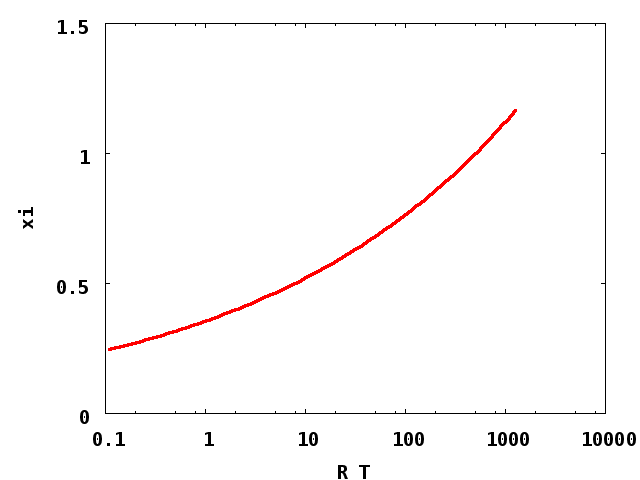
\includegraphics[width=7cm]{figures/FIG-xi3-xi}%
\lthtmlpictureZ
\lthtmlcheckvsize\clearpage}

{\newpage\clearpage
\lthtmlpictureA{tex2html_wrap3794}%
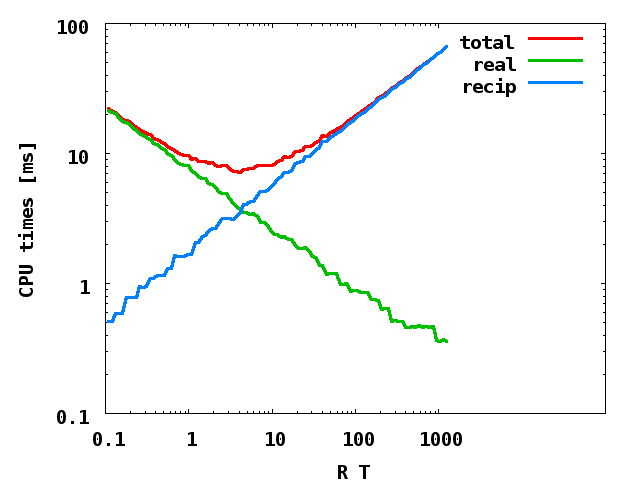
\includegraphics[width=7cm]{figures/FIG-xi3-CPU}%
\lthtmlpictureZ
\lthtmlcheckvsize\clearpage}

{\newpage\clearpage
\lthtmlinlinemathA{tex2html_wrap_inline3796}%
$ N=8$%
\lthtmlinlinemathZ
\lthtmlcheckvsize\clearpage}

{\newpage\clearpage
\lthtmlinlinemathA{tex2html_wrap_inline3798}%
$ (5, 5, 5)$%
\lthtmlinlinemathZ
\lthtmlcheckvsize\clearpage}

{\newpage\clearpage
\lthtmlinlinemathA{tex2html_wrap_inline3800}%
$ R_T\approx 4$%
\lthtmlinlinemathZ
\lthtmlcheckvsize\clearpage}

{\newpage\clearpage
\lthtmlinlinemathA{tex2html_wrap_inline3810}%
$ {\tt ewald\_eps} = 10^{-12}$%
\lthtmlinlinemathZ
\lthtmlcheckvsize\clearpage}

{\newpage\clearpage
\lthtmlinlinemathA{tex2html_wrap_inline3812}%
$ \mathbf{A}\cdot\mathbf{x}$%
\lthtmlinlinemathZ
\lthtmlcheckvsize\clearpage}

{\newpage\clearpage
\lthtmlinlinemathA{tex2html_wrap_inline3814}%
$ \mathbf{A}$%
\lthtmlinlinemathZ
\lthtmlcheckvsize\clearpage}

{\newpage\clearpage
\lthtmlinlinemathA{tex2html_wrap_inline3816}%
$ \mathbf{x} = (1,1,\cdots,1)^\dagger$%
\lthtmlinlinemathZ
\lthtmlcheckvsize\clearpage}

{\newpage\clearpage
\lthtmlpictureA{tex2html_wrap3822}%
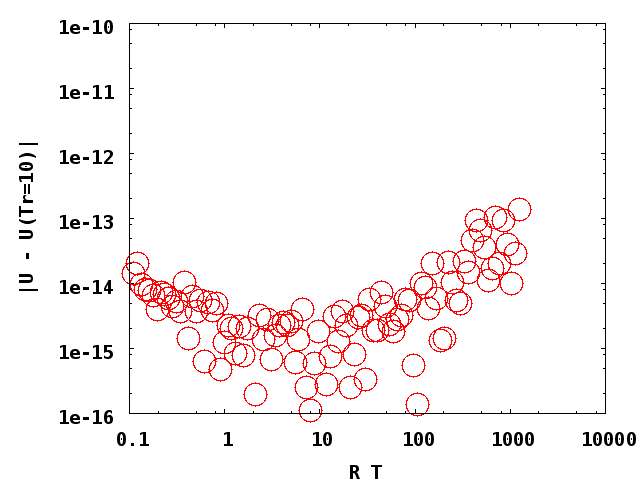
\includegraphics[width=7cm]{figures/FIG-xi3-err}%
\lthtmlpictureZ
\lthtmlcheckvsize\clearpage}

{\newpage\clearpage
\lthtmlinlinemathA{tex2html_wrap_inline3826}%
$ R_T \approx 10$%
\lthtmlinlinemathZ
\lthtmlcheckvsize\clearpage}

\stepcounter{subsection}
\stepcounter{section}
\stepcounter{section}
\stepcounter{subsection}
{\newpage\clearpage
\lthtmlinlinemathA{tex2html_wrap_inline3832}%
$ 10$%
\lthtmlinlinemathZ
\lthtmlcheckvsize\clearpage}

{\newpage\clearpage
\lthtmlinlinemathA{tex2html_wrap_inline3834}%
$ \bm{U} = (1,1,1)$%
\lthtmlinlinemathZ
\lthtmlcheckvsize\clearpage}

\stepcounter{subsection}
\stepcounter{subsection}
\stepcounter{subsection}
\stepcounter{subsection}
\stepcounter{subsection}
\stepcounter{chapter}
\stepcounter{section}
\stepcounter{subsection}
\stepcounter{paragraph}
\stepcounter{paragraph}
\stepcounter{subsection}
\stepcounter{paragraph}
\stepcounter{paragraph}
{\newpage\clearpage
\lthtmlinlinemathA{tex2html_wrap_inline3849}%
$ t=t_0$%
\lthtmlinlinemathZ
\lthtmlcheckvsize\clearpage}

{\newpage\clearpage
\lthtmlinlinemathA{tex2html_wrap_inline3851}%
$ t$%
\lthtmlinlinemathZ
\lthtmlcheckvsize\clearpage}

\stepcounter{subsection}
{\newpage\clearpage
\lthtmlinlinemathA{tex2html_wrap_indisplay3856}%
$\displaystyle {\tt void\quad solve\_\langle type\rangle\_\langle lub\rangle\_\langle d\rangle\langle ver\rangle\_\langle mat\rangle(sys,\  givens,\  unknowns);}$%
\lthtmlindisplaymathZ
\lthtmlcheckvsize\clearpage}

\stepcounter{paragraph}
{\newpage\clearpage
\lthtmlinlinemathA{tex2html_wrap_inline3859}%
$ \langle$%
\lthtmlinlinemathZ
\lthtmlcheckvsize\clearpage}

{\newpage\clearpage
\lthtmlinlinemathA{tex2html_wrap_inline3861}%
$ \rangle$%
\lthtmlinlinemathZ
\lthtmlcheckvsize\clearpage}

{\newpage\clearpage
\lthtmlinlinemathA{tex2html_wrap_inline3863}%
$ ({\tt u, o, e}) \mapsto ({\tt f, t, s})$%
\lthtmlinlinemathZ
\lthtmlcheckvsize\clearpage}

{\newpage\clearpage
\lthtmlinlinemathA{tex2html_wrap_inline3865}%
$ ({\tt f, t, e}) \mapsto ({\tt u, o, s})$%
\lthtmlinlinemathZ
\lthtmlcheckvsize\clearpage}

{\newpage\clearpage
\lthtmlinlinemathA{tex2html_wrap_inline3867}%
$ ({\tt f, t, e, uf, of, ef}) \mapsto ({\tt u, o, s, ff, tf, sf})$%
\lthtmlinlinemathZ
\lthtmlcheckvsize\clearpage}

\stepcounter{paragraph}
\stepcounter{paragraph}
\stepcounter{paragraph}
\stepcounter{paragraph}
\stepcounter{section}
{\newpage\clearpage
\lthtmlinlinemathA{tex2html_wrap_indisplay3894}%
$\displaystyle \frac{\partial}{\partial t}   \Bigl[     \rho     \bm{u}     +     \left(       \bm{u}       \cdot       \bm{\nabla}     \right)     \bm{u}   \Bigr]   =   -   \bm{\nabla}   p   +   \mu   \Delta   \bm{u}   ,$%
\lthtmlindisplaymathZ
\lthtmlcheckvsize\clearpage}

{\newpage\clearpage
\lthtmlinlinemathA{tex2html_wrap_inline3896}%
$ \bm{u}$%
\lthtmlinlinemathZ
\lthtmlcheckvsize\clearpage}

{\newpage\clearpage
\lthtmlinlinemathA{tex2html_wrap_inline3898}%
$ p$%
\lthtmlinlinemathZ
\lthtmlcheckvsize\clearpage}

{\newpage\clearpage
\lthtmlinlinemathA{tex2html_wrap_inline3900}%
$ \rho$%
\lthtmlinlinemathZ
\lthtmlcheckvsize\clearpage}

{\newpage\clearpage
\lthtmlinlinemathA{tex2html_wrap_indisplay3904}%
$\displaystyle \bm{\nabla}   =   \left[     \begin{array}{c}       \partial/\partial x\\\partial/\partial y\\\partial/\partial z     \end{array}   \right]   ,$%
\lthtmlindisplaymathZ
\lthtmlcheckvsize\clearpage}

{\newpage\clearpage
\lthtmlinlinemathA{tex2html_wrap_inline3906}%
$ \Delta$%
\lthtmlinlinemathZ
\lthtmlcheckvsize\clearpage}

{\newpage\clearpage
\lthtmlinlinemathA{tex2html_wrap_indisplay3908}%
$\displaystyle \Delta   =   \bm{\nabla}   \cdot   \bm{\nabla}   =   \partial^2/\partial x^2   +   \partial^2/\partial y^2   +   \partial^2/\partial z^2   .$%
\lthtmlindisplaymathZ
\lthtmlcheckvsize\clearpage}

{\newpage\clearpage
\lthtmlinlinemathA{tex2html_wrap_inline3910}%
$ \bm{F} = m\bm{a}$%
\lthtmlinlinemathZ
\lthtmlcheckvsize\clearpage}

{\newpage\clearpage
\lthtmlinlinemathA{tex2html_wrap_indisplay3912}%
$\displaystyle \bm{\sigma}   =   p   \bm{I}   +   \bm{\nabla}\bm{u}   +   \Bigl(   \bm{\nabla}\bm{u}   \Bigr)^\dagger   ,$%
\lthtmlindisplaymathZ
\lthtmlcheckvsize\clearpage}

{\newpage\clearpage
\lthtmlinlinemathA{tex2html_wrap_indisplay3914}%
$\displaystyle \frac{D}{D t}   \Bigl[     \rho     \bm{u}   \Bigr]   =   -   \bm{\nabla}   \cdot   \bm{\sigma}   .$%
\lthtmlindisplaymathZ
\lthtmlcheckvsize\clearpage}

{\newpage\clearpage
\lthtmlinlinemathA{tex2html_wrap_inline3916}%
$ Re$%
\lthtmlinlinemathZ
\lthtmlcheckvsize\clearpage}

{\newpage\clearpage
\lthtmlinlinemathA{tex2html_wrap_indisplay3918}%
$\displaystyle Re   :=   \frac{LU}{\mu}   ,$%
\lthtmlindisplaymathZ
\lthtmlcheckvsize\clearpage}

{\newpage\clearpage
\lthtmlinlinemathA{tex2html_wrap_inline3920}%
$ L$%
\lthtmlinlinemathZ
\lthtmlcheckvsize\clearpage}

{\newpage\clearpage
\lthtmlinlinemathA{tex2html_wrap_inline3922}%
$ U$%
\lthtmlinlinemathZ
\lthtmlcheckvsize\clearpage}

{\newpage\clearpage
\lthtmlinlinemathA{tex2html_wrap_inline3924}%
$ Re\rightarrow 0$%
\lthtmlinlinemathZ
\lthtmlcheckvsize\clearpage}

{\newpage\clearpage
\lthtmlinlinemathA{tex2html_wrap_indisplay3926}%
$\displaystyle \bm{0}   =   -   \bm{\nabla}   p   +   \mu   \Delta   \bm{u}   ,$%
\lthtmlindisplaymathZ
\lthtmlcheckvsize\clearpage}

{\newpage\clearpage
\lthtmlinlinemathA{tex2html_wrap_indisplay3928}%
$\displaystyle \bm{\nabla}   \cdot   \bm{u}   =   0   .$%
\lthtmlindisplaymathZ
\lthtmlcheckvsize\clearpage}

\stepcounter{subsection}
{\newpage\clearpage
\lthtmlinlinemathA{tex2html_wrap_indisplay3931}%
$\displaystyle \bm{u}   (\bm{x})   =   -   \frac{1}{8\pi\mu}   \int_S   {\rm d}S(\bm{y})\     \bm{J}(\bm{x}-\bm{y})   \cdot   \bm{f}(\bm{y})   .$%
\lthtmlindisplaymathZ
\lthtmlcheckvsize\clearpage}

{\newpage\clearpage
\lthtmlinlinemathA{tex2html_wrap_indisplay3933}%
$\displaystyle \bm{u}   (\bm{x})   =   -   \frac{1}{n!}   \sum_{n=0}^{\infty}   \frac{1}{8\pi\mu}   \Bigl[     (-)^n     \bm{\nabla}^n     \bm{J}   \Bigr]   (\bm{x}-\bm{y}_0)   \odot^n   \int_S   {\rm d}S(\bm{y})\     \Bigl[     \bm{y}     -     \bm{y}_0   \Bigr]^n   \bm{f}(\bm{y})   ,$%
\lthtmlindisplaymathZ
\lthtmlcheckvsize\clearpage}

{\newpage\clearpage
\lthtmlinlinemathA{tex2html_wrap_inline3935}%
$ S$%
\lthtmlinlinemathZ
\lthtmlcheckvsize\clearpage}

{\newpage\clearpage
\lthtmlinlinemathA{tex2html_wrap_inline3937}%
$ \bm{y}_0$%
\lthtmlinlinemathZ
\lthtmlcheckvsize\clearpage}

{\newpage\clearpage
\lthtmlinlinemathA{tex2html_wrap_inline3939}%
$ (n+1)$%
\lthtmlinlinemathZ
\lthtmlcheckvsize\clearpage}

{\newpage\clearpage
\lthtmlinlinemathA{tex2html_wrap_inline3941}%
$ \mathcal{F}^{(n)}$%
\lthtmlinlinemathZ
\lthtmlcheckvsize\clearpage}

{\newpage\clearpage
\lthtmlinlinemathA{tex2html_wrap_indisplay3943}%
$\displaystyle \mathcal{F}^{(n)}   (\bm{y}_0)   :=   -   \int_S   {\rm d}S(\bm{y})\     \Bigl[     \bm{y}     -     \bm{y}_0   \Bigr]^n   \bm{f}(\bm{y})   ,$%
\lthtmlindisplaymathZ
\lthtmlcheckvsize\clearpage}

{\newpage\clearpage
\lthtmlinlinemathA{tex2html_wrap_indisplay3946}%
$\displaystyle \mathcal{F}^{(0)}
(\bm{y}_0)$%
\lthtmlindisplaymathZ
\lthtmlcheckvsize\clearpage}

{\newpage\clearpage
\lthtmlinlinemathA{tex2html_wrap_indisplay3950}%
$\displaystyle \bm{F}
,$%
\lthtmlindisplaymathZ
\lthtmlcheckvsize\clearpage}

{\newpage\clearpage
\lthtmlinlinemathA{tex2html_wrap_indisplay3952}%
$\displaystyle \mathcal{F}^{(1)}
(\bm{y}_0)$%
\lthtmlindisplaymathZ
\lthtmlcheckvsize\clearpage}

{\newpage\clearpage
\lthtmlinlinemathA{tex2html_wrap_indisplay3956}%
$\displaystyle \bm{\epsilon}
\cdot
\bm{T}
+
\bm{S}
.$%
\lthtmlindisplaymathZ
\lthtmlcheckvsize\clearpage}

{\newpage\clearpage
\lthtmlinlinemathA{tex2html_wrap_inline3958}%
$ n=1$%
\lthtmlinlinemathZ
\lthtmlcheckvsize\clearpage}

{\newpage\clearpage
\lthtmlinlinemathA{tex2html_wrap_indisplay3960}%
$\displaystyle \bm{u}   (\bm{x})   =   \Bigl(     1     +     \frac{a^2\nabla^2}{6}   \Bigr)   \bm{J}   (\bm{x}-\bm{y}_0)   \cdot   \bm{F}   +   \bm{R}   (\bm{x}-\bm{y}_0)   \cdot   \bm{T}   -   \Bigl(     1     +     \frac{a^2\nabla^2}{10}   \Bigr)   \bm{K}   (\bm{x}-\bm{y}_0)   \odot^2   \bm{S}   ,$%
\lthtmlindisplaymathZ
\lthtmlcheckvsize\clearpage}

{\newpage\clearpage
\lthtmlinlinemathA{tex2html_wrap_inline3962}%
$ \bm{R}$%
\lthtmlinlinemathZ
\lthtmlcheckvsize\clearpage}

{\newpage\clearpage
\lthtmlinlinemathA{tex2html_wrap_inline3964}%
$ \bm{K}$%
\lthtmlinlinemathZ
\lthtmlcheckvsize\clearpage}

{\newpage\clearpage
\lthtmlinlinemathA{tex2html_wrap_indisplay3967}%
$\displaystyle \bm{R}$%
\lthtmlindisplaymathZ
\lthtmlcheckvsize\clearpage}

{\newpage\clearpage
\lthtmlinlinemathA{tex2html_wrap_indisplay3971}%
$\displaystyle ,$%
\lthtmlindisplaymathZ
\lthtmlcheckvsize\clearpage}

{\newpage\clearpage
\lthtmlinlinemathA{tex2html_wrap_indisplay3973}%
$\displaystyle \bm{K}$%
\lthtmlindisplaymathZ
\lthtmlcheckvsize\clearpage}

{\newpage\clearpage
\lthtmlinlinemathA{tex2html_wrap_indisplay3977}%
$\displaystyle .$%
\lthtmlindisplaymathZ
\lthtmlcheckvsize\clearpage}

{\newpage\clearpage
\lthtmlinlinemathA{tex2html_wrap_inline3981}%
$ \bm{\Omega}$%
\lthtmlinlinemathZ
\lthtmlcheckvsize\clearpage}

{\newpage\clearpage
\lthtmlinlinemathA{tex2html_wrap_inline3983}%
$ \bm{E}$%
\lthtmlinlinemathZ
\lthtmlcheckvsize\clearpage}

{\newpage\clearpage
\lthtmlinlinemathA{tex2html_wrap_indisplay3985}%
$\displaystyle \left[     \begin{array}{c}       \bm{U}\\\bm{\Omega}\\\bm{E}     \end{array}   \right]   =   \left[     \begin{array}{ccc}       \bm{a} & \bm{b} & \bm{g}\\\tilde{\bm{b}} & \bm{c} & \bm{h}\\\tilde{\bm{g}} & \tilde{h} & \bm{m}     \end{array}   \right]   \cdot   \left[     \begin{array}{c}       \bm{F}\\\bm{T}\\\bm{S}     \end{array}   \right]   .$%
\lthtmlindisplaymathZ
\lthtmlcheckvsize\clearpage}

{\newpage\clearpage
\lthtmlinlinemathA{tex2html_wrap_inline3987}%
$ (\bm{U}, \bm{\Omega}, \bm{E})^\dagger$%
\lthtmlinlinemathZ
\lthtmlcheckvsize\clearpage}

{\newpage\clearpage
\lthtmlinlinemathA{tex2html_wrap_inline3989}%
$ (\bm{F}, \bm{T}, \bm{S})^\dagger$%
\lthtmlinlinemathZ
\lthtmlcheckvsize\clearpage}

{\newpage\clearpage
\lthtmlinlinemathA{tex2html_wrap_indisplay3992}%
$\displaystyle a_{ij}$%
\lthtmlindisplaymathZ
\lthtmlcheckvsize\clearpage}

{\newpage\clearpage
\lthtmlinlinemathA{tex2html_wrap_indisplay3996}%
$\displaystyle a_{ji},$%
\lthtmlindisplaymathZ
\lthtmlcheckvsize\clearpage}

{\newpage\clearpage
\lthtmlinlinemathA{tex2html_wrap_indisplay3998}%
$\displaystyle \tilde{b}_{ij}$%
\lthtmlindisplaymathZ
\lthtmlcheckvsize\clearpage}

{\newpage\clearpage
\lthtmlinlinemathA{tex2html_wrap_indisplay4002}%
$\displaystyle b_{ji},$%
\lthtmlindisplaymathZ
\lthtmlcheckvsize\clearpage}

{\newpage\clearpage
\lthtmlinlinemathA{tex2html_wrap_indisplay4004}%
$\displaystyle c_{ij}$%
\lthtmlindisplaymathZ
\lthtmlcheckvsize\clearpage}

{\newpage\clearpage
\lthtmlinlinemathA{tex2html_wrap_indisplay4008}%
$\displaystyle c_{ji}.$%
\lthtmlindisplaymathZ
\lthtmlcheckvsize\clearpage}

{\newpage\clearpage
\lthtmlinlinemathA{tex2html_wrap_inline4012}%
$ \bm{S}$%
\lthtmlinlinemathZ
\lthtmlcheckvsize\clearpage}

{\newpage\clearpage
\lthtmlinlinemathA{tex2html_wrap_inline4014}%
$ 3\times 3$%
\lthtmlinlinemathZ
\lthtmlcheckvsize\clearpage}

\stepcounter{paragraph}
\stepcounter{subsection}
{\newpage\clearpage
\lthtmlinlinemathA{tex2html_wrap_inline4024}%
$ \bm{F}$%
\lthtmlinlinemathZ
\lthtmlcheckvsize\clearpage}

{\newpage\clearpage
\lthtmlinlinemathA{tex2html_wrap_inline4026}%
$ \bm{T}$%
\lthtmlinlinemathZ
\lthtmlcheckvsize\clearpage}

{\newpage\clearpage
\lthtmlinlinemathA{tex2html_wrap_indisplay4050}%
$\displaystyle \left[     \begin{array}{c}       \bm{U}\\\bm{\Omega}\\\bm{S}     \end{array}   \right]   =   \bm{M}'   \cdot   \left[     \begin{array}{c}       \bm{F}\\\bm{T}\\\bm{E}     \end{array}   \right]   .$%
\lthtmlindisplaymathZ
\lthtmlcheckvsize\clearpage}

{\newpage\clearpage
\lthtmlinlinemathA{tex2html_wrap_indisplay4053}%
$\displaystyle {\bm{M}'}_{UF}$%
\lthtmlindisplaymathZ
\lthtmlcheckvsize\clearpage}

{\newpage\clearpage
\lthtmlinlinemathA{tex2html_wrap_indisplay4057}%
$\displaystyle \bm{M}_{UF}
-
\bm{M}_{US}
\cdot
\Bigl(
\bm{M}_{ES}
\Bigr)^{-1}
\cdot
\bm{M}_{EF}
,$%
\lthtmlindisplaymathZ
\lthtmlcheckvsize\clearpage}

{\newpage\clearpage
\lthtmlinlinemathA{tex2html_wrap_indisplay4059}%
$\displaystyle {\bm{M}'}_{UE}$%
\lthtmlindisplaymathZ
\lthtmlcheckvsize\clearpage}

{\newpage\clearpage
\lthtmlinlinemathA{tex2html_wrap_indisplay4063}%
$\displaystyle \bm{M}_{US}
\cdot
\Bigl(
\bm{M}_{ES}
\Bigr)^{-1}
,$%
\lthtmlindisplaymathZ
\lthtmlcheckvsize\clearpage}

{\newpage\clearpage
\lthtmlinlinemathA{tex2html_wrap_indisplay4065}%
$\displaystyle {\bm{M}'}_{SF}$%
\lthtmlindisplaymathZ
\lthtmlcheckvsize\clearpage}

{\newpage\clearpage
\lthtmlinlinemathA{tex2html_wrap_indisplay4069}%
$\displaystyle -
\Bigl(
\bm{M}_{ES}
\Bigr)^{-1}
\cdot
\bm{M}_{EF}
,$%
\lthtmlindisplaymathZ
\lthtmlcheckvsize\clearpage}

{\newpage\clearpage
\lthtmlinlinemathA{tex2html_wrap_indisplay4071}%
$\displaystyle {\bm{M}'}_{SE}$%
\lthtmlindisplaymathZ
\lthtmlcheckvsize\clearpage}

{\newpage\clearpage
\lthtmlinlinemathA{tex2html_wrap_indisplay4075}%
$\displaystyle \Bigl(
\bm{M}_{ES}
\Bigr)^{-1}
,$%
\lthtmlindisplaymathZ
\lthtmlcheckvsize\clearpage}

{\newpage\clearpage
\lthtmlinlinemathA{tex2html_wrap_indisplay4077}%
$\displaystyle \left[     \begin{array}{c}       \bm{U}\\\bm{S}     \end{array}   \right]   =   \left[     \begin{array}{cc}       {\bm{M}'}_{UF} & {\bm{M}'}_{UE}\\{\bm{M}'}_{SF} & {\bm{M}'}_{SE}     \end{array}   \right]   \cdot   \left[     \begin{array}{c}       \bm{F}\\\bm{E}     \end{array}   \right]   ,$%
\lthtmlindisplaymathZ
\lthtmlcheckvsize\clearpage}

{\newpage\clearpage
\lthtmlinlinemathA{tex2html_wrap_indisplay4079}%
$\displaystyle \left[     \begin{array}{c}       \bm{U}\\\bm{E}     \end{array}   \right]   =   \left[     \begin{array}{cc}       \bm{M}_{UF} & \bm{M}_{US}\\\bm{M}_{EF} & \bm{M}_{ES}     \end{array}   \right]   \cdot   \left[     \begin{array}{c}       \bm{F}\\\bm{S}     \end{array}   \right]   .$%
\lthtmlindisplaymathZ
\lthtmlcheckvsize\clearpage}

\stepcounter{subsection}
{\newpage\clearpage
\lthtmlinlinemathA{tex2html_wrap_indisplay4092}%
$\displaystyle \left[     \begin{array}{c}       \bm{U}^{m}\\\bm{E}^{m}\\\bm{U}^{f}\\\bm{E}^{f}     \end{array}   \right]   =   \left[     \begin{array}{cccc}       \bm{M}_{UF}^{mm} & \bm{M}_{US}^{mm} & \bm{M}_{UF}^{mf} & \bm{M}_{US}^{mf}\\\bm{M}_{EF}^{mm} & \bm{M}_{ES}^{mm} & \bm{M}_{EF}^{mf} & \bm{M}_{ES}^{mf}\\\bm{M}_{UF}^{fm} & \bm{M}_{US}^{fm} & \bm{M}_{UF}^{ff} & \bm{M}_{US}^{ff}\\\bm{M}_{EF}^{fm} & \bm{M}_{ES}^{fm} & \bm{M}_{EF}^{ff} & \bm{M}_{ES}^{ff}\\\end{array}   \right]   \cdot   \left[     \begin{array}{c}       \bm{F}^{m}\\\bm{S}^{m}\\\bm{F}^{f}\\\bm{S}^{f}     \end{array}   \right]   .$%
\lthtmlindisplaymathZ
\lthtmlcheckvsize\clearpage}

{\newpage\clearpage
\lthtmlinlinemathA{tex2html_wrap_inline4094}%
$ m$%
\lthtmlinlinemathZ
\lthtmlcheckvsize\clearpage}

{\newpage\clearpage
\lthtmlinlinemathA{tex2html_wrap_inline4096}%
$ f$%
\lthtmlinlinemathZ
\lthtmlcheckvsize\clearpage}

{\newpage\clearpage
\lthtmlinlinemathA{tex2html_wrap_indisplay4098}%
$\displaystyle \bm{B}   \cdot   \left[     \begin{array}{c}       \bm{F}^{m}\\\bm{E}^{m}\\\bm{U}^{f}\\\bm{E}^{f}     \end{array}   \right]   =   \bm{A}   \cdot   \left[     \begin{array}{c}       \bm{U}^{m}\\\bm{S}^{m}\\\bm{F}^{f}\\\bm{S}^{f}     \end{array}   \right]   ,$%
\lthtmlindisplaymathZ
\lthtmlcheckvsize\clearpage}

{\newpage\clearpage
\lthtmlinlinemathA{tex2html_wrap_inline4100}%
$ \bm{A}$%
\lthtmlinlinemathZ
\lthtmlcheckvsize\clearpage}

{\newpage\clearpage
\lthtmlinlinemathA{tex2html_wrap_inline4102}%
$ \bm{B}$%
\lthtmlinlinemathZ
\lthtmlcheckvsize\clearpage}

{\newpage\clearpage
\lthtmlinlinemathA{tex2html_wrap_inline4104}%
$ \bm{M}$%
\lthtmlinlinemathZ
\lthtmlcheckvsize\clearpage}

{\newpage\clearpage
\lthtmlinlinemathA{tex2html_wrap_indisplay4106}%
$\displaystyle \left[     \begin{array}{cccc}       -\bm{M}_{UF}^{mm} & \bm{0} & \bm{0} & \bm{0}\\-\bm{M}_{EF}^{mm} & \bm{I} & \bm{0} & \bm{0}\\-\bm{M}_{UF}^{fm} & \bm{0} & \bm{I} & \bm{0}\\-\bm{M}_{EF}^{fm} & \bm{0} & \bm{0} & \bm{I}\\\end{array}   \right]   \cdot   \left[     \begin{array}{c}       \bm{F}^{m}\\\bm{E}^{m}\\\bm{U}^{f}\\\bm{E}^{f}     \end{array}   \right]   =   \left[     \begin{array}{cccc}       -\bm{I} & \bm{M}_{US}^{mm} & \bm{M}_{UF}^{mf} & \bm{M}_{US}^{mf}\\\bm{0}  & \bm{M}_{ES}^{mm} & \bm{M}_{EF}^{mf} & \bm{M}_{ES}^{mf}\\\bm{0}  & \bm{M}_{US}^{fm} & \bm{M}_{UF}^{ff} & \bm{M}_{US}^{ff}\\\bm{0}  & \bm{M}_{ES}^{fm} & \bm{M}_{EF}^{ff} & \bm{M}_{ES}^{ff}\\\end{array}   \right]   \cdot   \left[     \begin{array}{c}       \bm{U}^{m}\\\bm{S}^{m}\\\bm{F}^{f}\\\bm{S}^{f}     \end{array}   \right]   .$%
\lthtmlindisplaymathZ
\lthtmlcheckvsize\clearpage}

{\newpage\clearpage
\lthtmlinlinemathA{tex2html_wrap_inline4112}%
$ \bm{b} = \bm{B}\cdot\bm{b}'$%
\lthtmlinlinemathZ
\lthtmlcheckvsize\clearpage}

{\newpage\clearpage
\lthtmlinlinemathA{tex2html_wrap_inline4116}%
$ 3\times 3 = 9$%
\lthtmlinlinemathZ
\lthtmlcheckvsize\clearpage}

\stepcounter{subsection}
{\newpage\clearpage
\lthtmlinlinemathA{tex2html_wrap_indisplay4119}%
$\displaystyle \bm{R}   \simeq   \left(     \bm{M}   \right)^{-1}   +   \bm{L}   .$%
\lthtmlindisplaymathZ
\lthtmlcheckvsize\clearpage}

{\newpage\clearpage
\lthtmlinlinemathA{tex2html_wrap_indisplay4123}%
$\displaystyle \Bigl(     \bm{I}     +     \bm{M}     \cdot     \bm{L}   \Bigr)   \cdot   \bm{U}   =   \bm{M}   \cdot   \bm{F}   ,$%
\lthtmlindisplaymathZ
\lthtmlcheckvsize\clearpage}

\stepcounter{subsection}
{\newpage\clearpage
\lthtmlinlinemathA{tex2html_wrap_inline4130}%
$ \bm{J}$%
\lthtmlinlinemathZ
\lthtmlcheckvsize\clearpage}

\stepcounter{subsection}
\stepcounter{section}
\stepcounter{section}
\stepcounter{subsection}
\stepcounter{subsection}
\stepcounter{subsection}
\stepcounter{subsection}
\stepcounter{subsection}
\stepcounter{section}
\stepcounter{chapter}
\stepcounter{section}
\stepcounter{section}
\stepcounter{section}
\stepcounter{chapter}
\stepcounter{section}
\stepcounter{section}
\stepcounter{section}
\stepcounter{section}
\stepcounter{chapter}
\stepcounter{chapter}
\appendix
\stepcounter{chapter}
\stepcounter{paragraph}
\addtocounter{enumi}{-1}

\end{document}
